% Euclidean Handout Number seventeen
\documentclass{tufte-handout}

%\geometry{showframe}% for debugging purposes -- displays the margins

%%%% Packages to make things pretty
\usepackage{amsmath,amsthm}
\usepackage{booktabs}
\usepackage{graphicx}
\setkeys{Gin}{width=\linewidth,totalheight=\textheight,keepaspectratio}
\graphicspath{{graphics/}}
\usepackage{units}
\usepackage{fancyvrb}
\fvset{fontsize=\normalsize}
\usepackage{multicol}
\usepackage{pdfpages}

%%%% Theorem Evironments
\theoremstyle{definition}
\swapnumbers
\newtheorem{problem}{Problem}[section]
\newtheorem{conjecture}[problem]{Conjecture}
\newtheorem*{definition}{Definition}
\newtheorem*{theorem}{Theorem}
\newtheorem{question}[problem]{Question}
\newtheorem{challenge}[problem]{Challenge}
\newtheorem*{postulate}{Postulate}

%%%%%

\title{Euclidean Geometry:\\An Introduction to Mathematical Work}
\author[]{Math 3600}
\date{Fall 2015}

\begin{document}

\maketitle

\begin{marginfigure}
    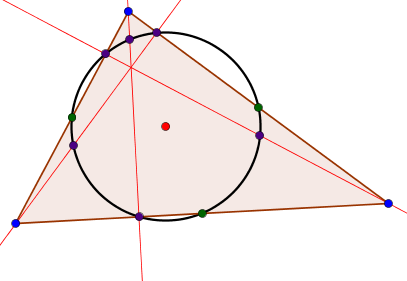
\includegraphics{NPC}
\end{marginfigure}

\setcounter{section}{17}
\section{More Triangle Centers}

Now it is time to play. We have studied lots of interesting topics, and we can use our understanding to prove beautiful theorems.

\begin{conjecture} Let $ABC$ be a triangle with $D$ the midpoint of $AB$ and $E$ the midpoint of $AC$. Then $BC$ is twice $DE$.
\end{conjecture}

\begin{definition}\label{defn:median}
Let $ABC$ be a triangle, and let $D$ be the midpoint of side $BC$. The segment $AD$ is called the \emph{median} of $ABC$ at $A$.
\end{definition}

\begin{conjecture}\label{conj:location-median}
Suppose that $m$ and $\ell $ are two medians of a triangle $ABC$.  The point where $m$ and $\ell$ intersect lies on each median $2/3$ of the way from the vertex to the opposite side.
\end{conjecture}

\begin{conjecture}\label{conj:medians-concurrent}
The medians of a triangle are concurrent.
\end{conjecture}

\begin{definition}\label{defn:centroid}
The point just found is called the \emph{centroid} of the triangle.
\end{definition}

%\begin{challenge}\label{chal:trisect-segment}
%Given a segment $AB$, find a point $M$ which lies on the segment such that if $a$ is the class of $AM$, then $a+a+a$ is the class of $AB$.
%(i.e. \emph{trisect} the segment.)
%\end{challenge}
%
%\begin{challenge}\label{chal:triangle-given-medians}
%Given three line segments, give a straightedge and compass construction of a triangle having medians congruent to the three given segments. How often is this construction possible?
%\end{challenge}

\begin{definition}\label{defn:altitude} Let $ABC$ be a triangle. A line from a vertex which is perpendicular to the opposite side is called an \emph{altitude}.
\end{definition}

\begin{definition}\label{defn:medial-triangle} Let $ABC$ be a triangle. The triangle formed by joining the midpoints of the sides of $ABC$ by segments is called the \emph{medial triangle} of $ABC$.
\end{definition}

\begin{conjecture} Let $ABC$ be a triangle with $DEF$ its medial triangle. An altitude of $DEF$ is a perpendicular bisector of one of the sides of $ABC$.
\end{conjecture}

\begin{conjecture}\label{conj:altitudes-concurrent} The three altitudes of a triangle are concurrent.
\end{conjecture}

\begin{definition}\label{defn:orthocenter} The point of concurrence of the altitudes of a triangle is called the \emph{orthocenter} of the triangle. The traditional notation is to label this point $H$.
\end{definition}

\marginnote[-225pt]{
A many hundreds of notions of what could be the ``center'' of a triangle have been investigated. A detailed list is compiled at the web page \url{http://faculty.evansville.edu/ck6/tcenters/}.}

\begin{problem}\label{prob:Euler-line}
Let $ABC$ be a triangle with circumcenter $O$, centroid $G$ and orthocenter $H$. Show that $O, H$ and $G$ are collinear, and $GH$ is twice $OG$.
\end{problem}

\begin{definition}\label{defn:Euler-line}
The line found in the last problem is called the \emph{Euler line} of triangle $ABC$.
\end{definition}


\vfill
\end{document}
